\begin{frame}
\frametitle{EyesOnCrops: iOS App journey}
% in documenet
\begin{itemize}
    \item Database Architecture 
    \item Wireframes \& UML Diagrams
    \item Front-end of the application
    \item Back-end of the application
    \item Using the application
    \item Data Analysis
\end{itemize}
\end{frame}

\begin{frame}
\frametitle{Database Information}
\begin{itemize}
    \item PostgreSQL database used
    \item PHP has been used to make SQL queries.
    \item Three tables created which are as follows:
\end{itemize}
 \begin{itemize}
        \item Users
        \item role\_master
        \item masked\_ndvi
    \end{itemize}
\end{frame}

\begin{frame}
\frametitle{Database tables}
\begin{figure}
    \centering
    \begin{minipage}{0.75\columnwidth}
    %\includegraphics[width=\linewidth]{ts-compare.png}
    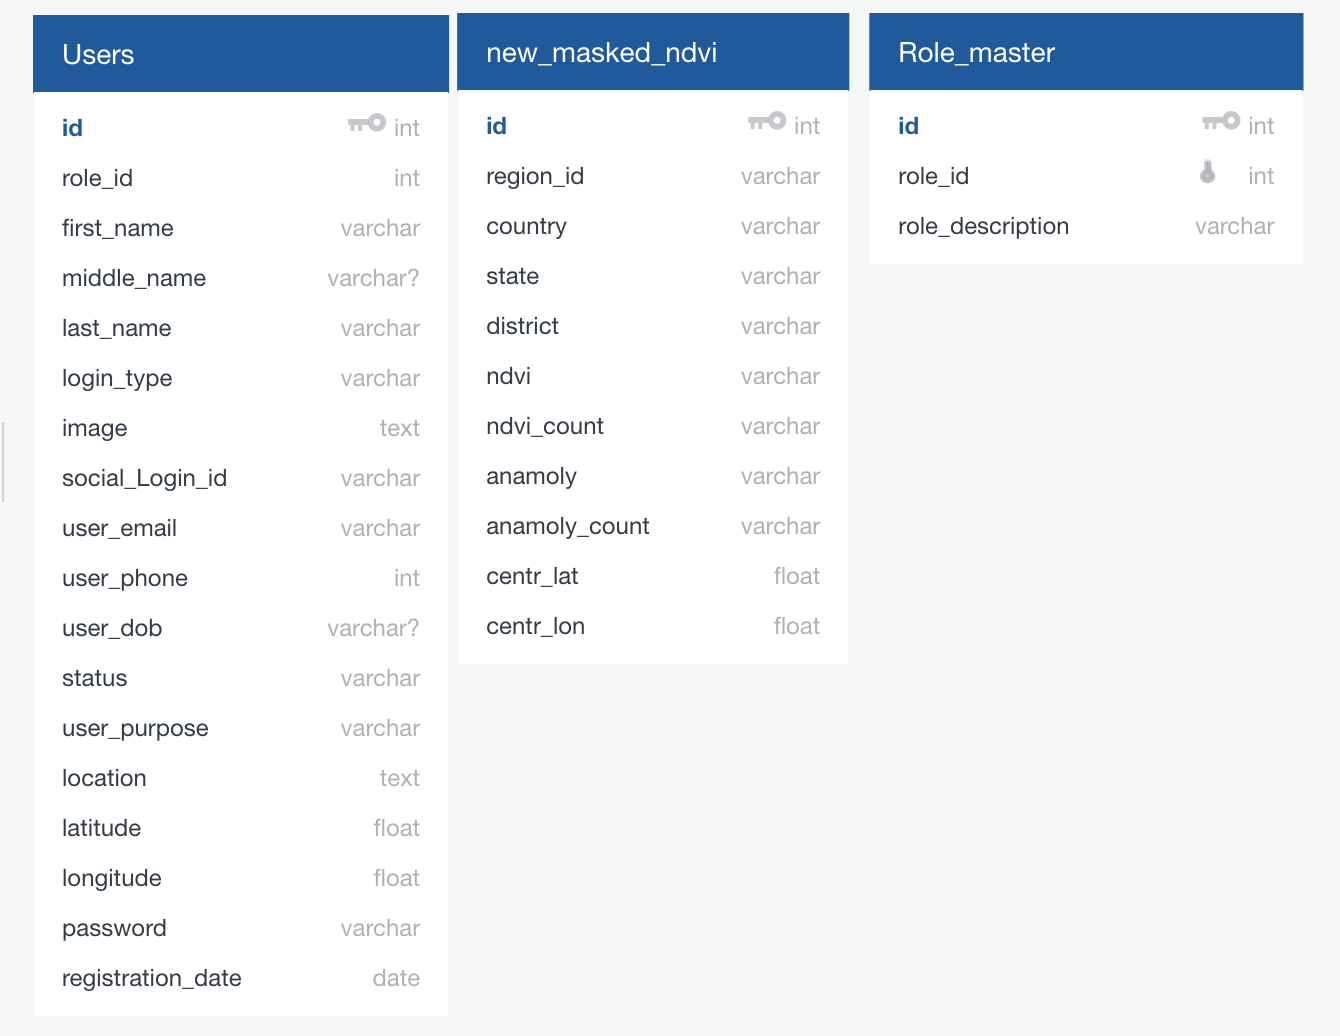
\includegraphics[width=\linewidth]{final/figures/database_structure.png}
    \caption{\tiny{Database tables)}}
    \end{minipage}
\end{figure}
\end{frame}



\begin{frame}
\frametitle{Wireframes \& UML diagrams}
\begin{itemize}
    \item A skeletal of the project
    \item Used to visualize the app screens and their flow.
    \item UML: Unified modeling language: a modern approach to modeling and documenting software.
    \item Helps developers to analyze the product efficiently.
    \item Use case diagram and class diagram has been created for the above purpose.
\end{itemize}

\end{frame}

\begin{frame}
\frametitle{Wireframes sample design}
 \begin{figure}[H]
            \centering
            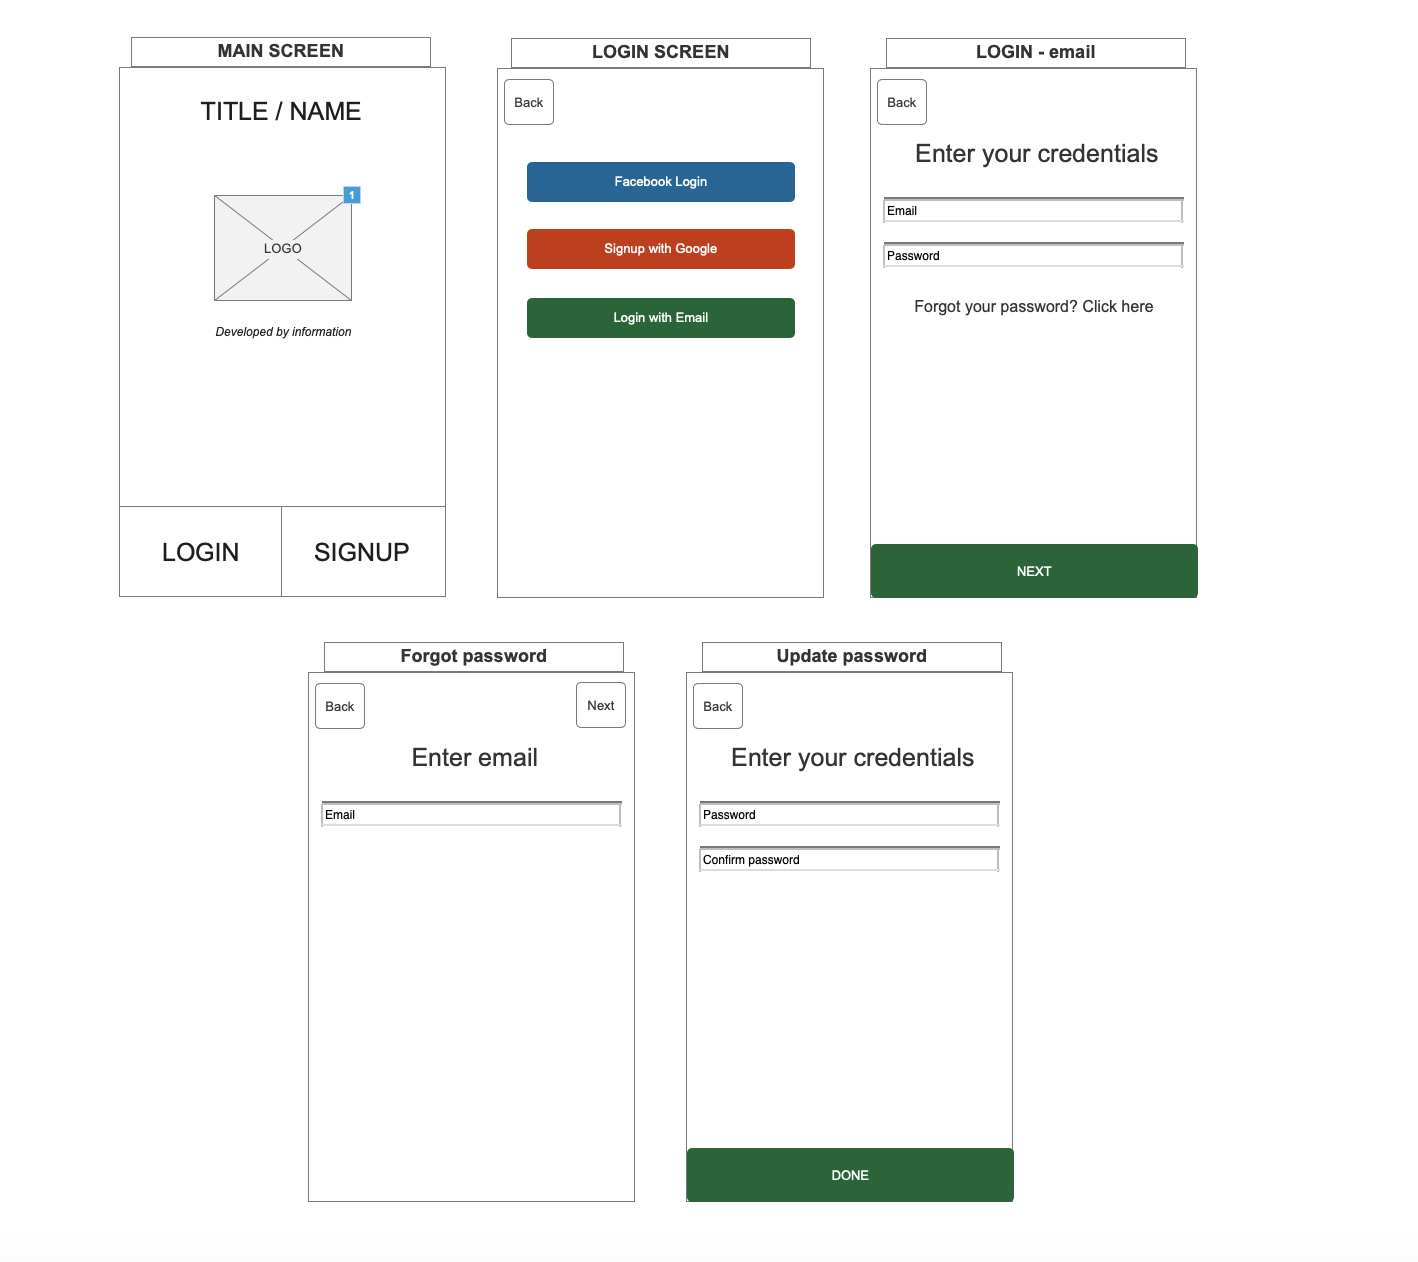
\includegraphics[width=0.60\linewidth]{figures/wireframe_2.png}
            \caption{Wireframe design}
    \end{figure}
\end{frame}

\begin{frame}
\frametitle{Use Case diagram describing functionality of the product}
 \begin{figure}[H]
            \centering
            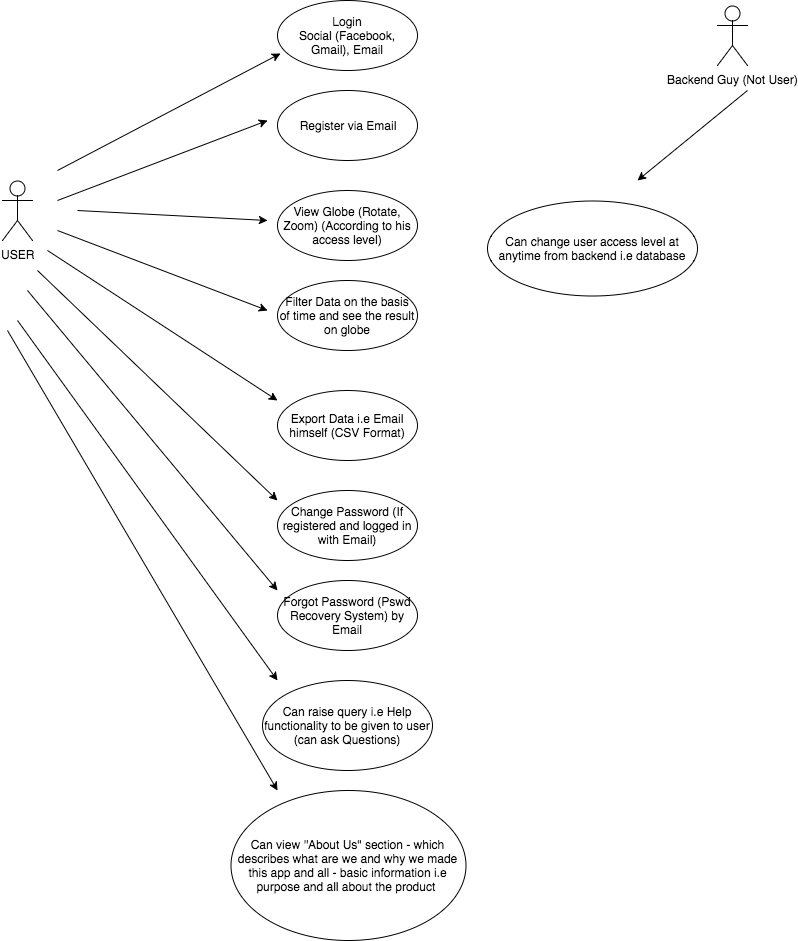
\includegraphics[width=0.50\linewidth]{final/figures/usecase.png}
            \caption{Use case diagram describing functionality of the product}
    \end{figure}
\end{frame}


\begin{frame}
\frametitle{Front-end of the application: App Design}
 \begin{itemize}
    \item Storyboard: Apple's Interface builder used for designing the front-end. 
    \item A container for all the scenes
    \item A manager of connections and transitions between these scenes (these are called Segues)
\end{itemize}
\end{frame}

\begin{frame}
\frametitle{Front-end: Storyboard of the app}
 \begin{figure}[H]
            \centering
            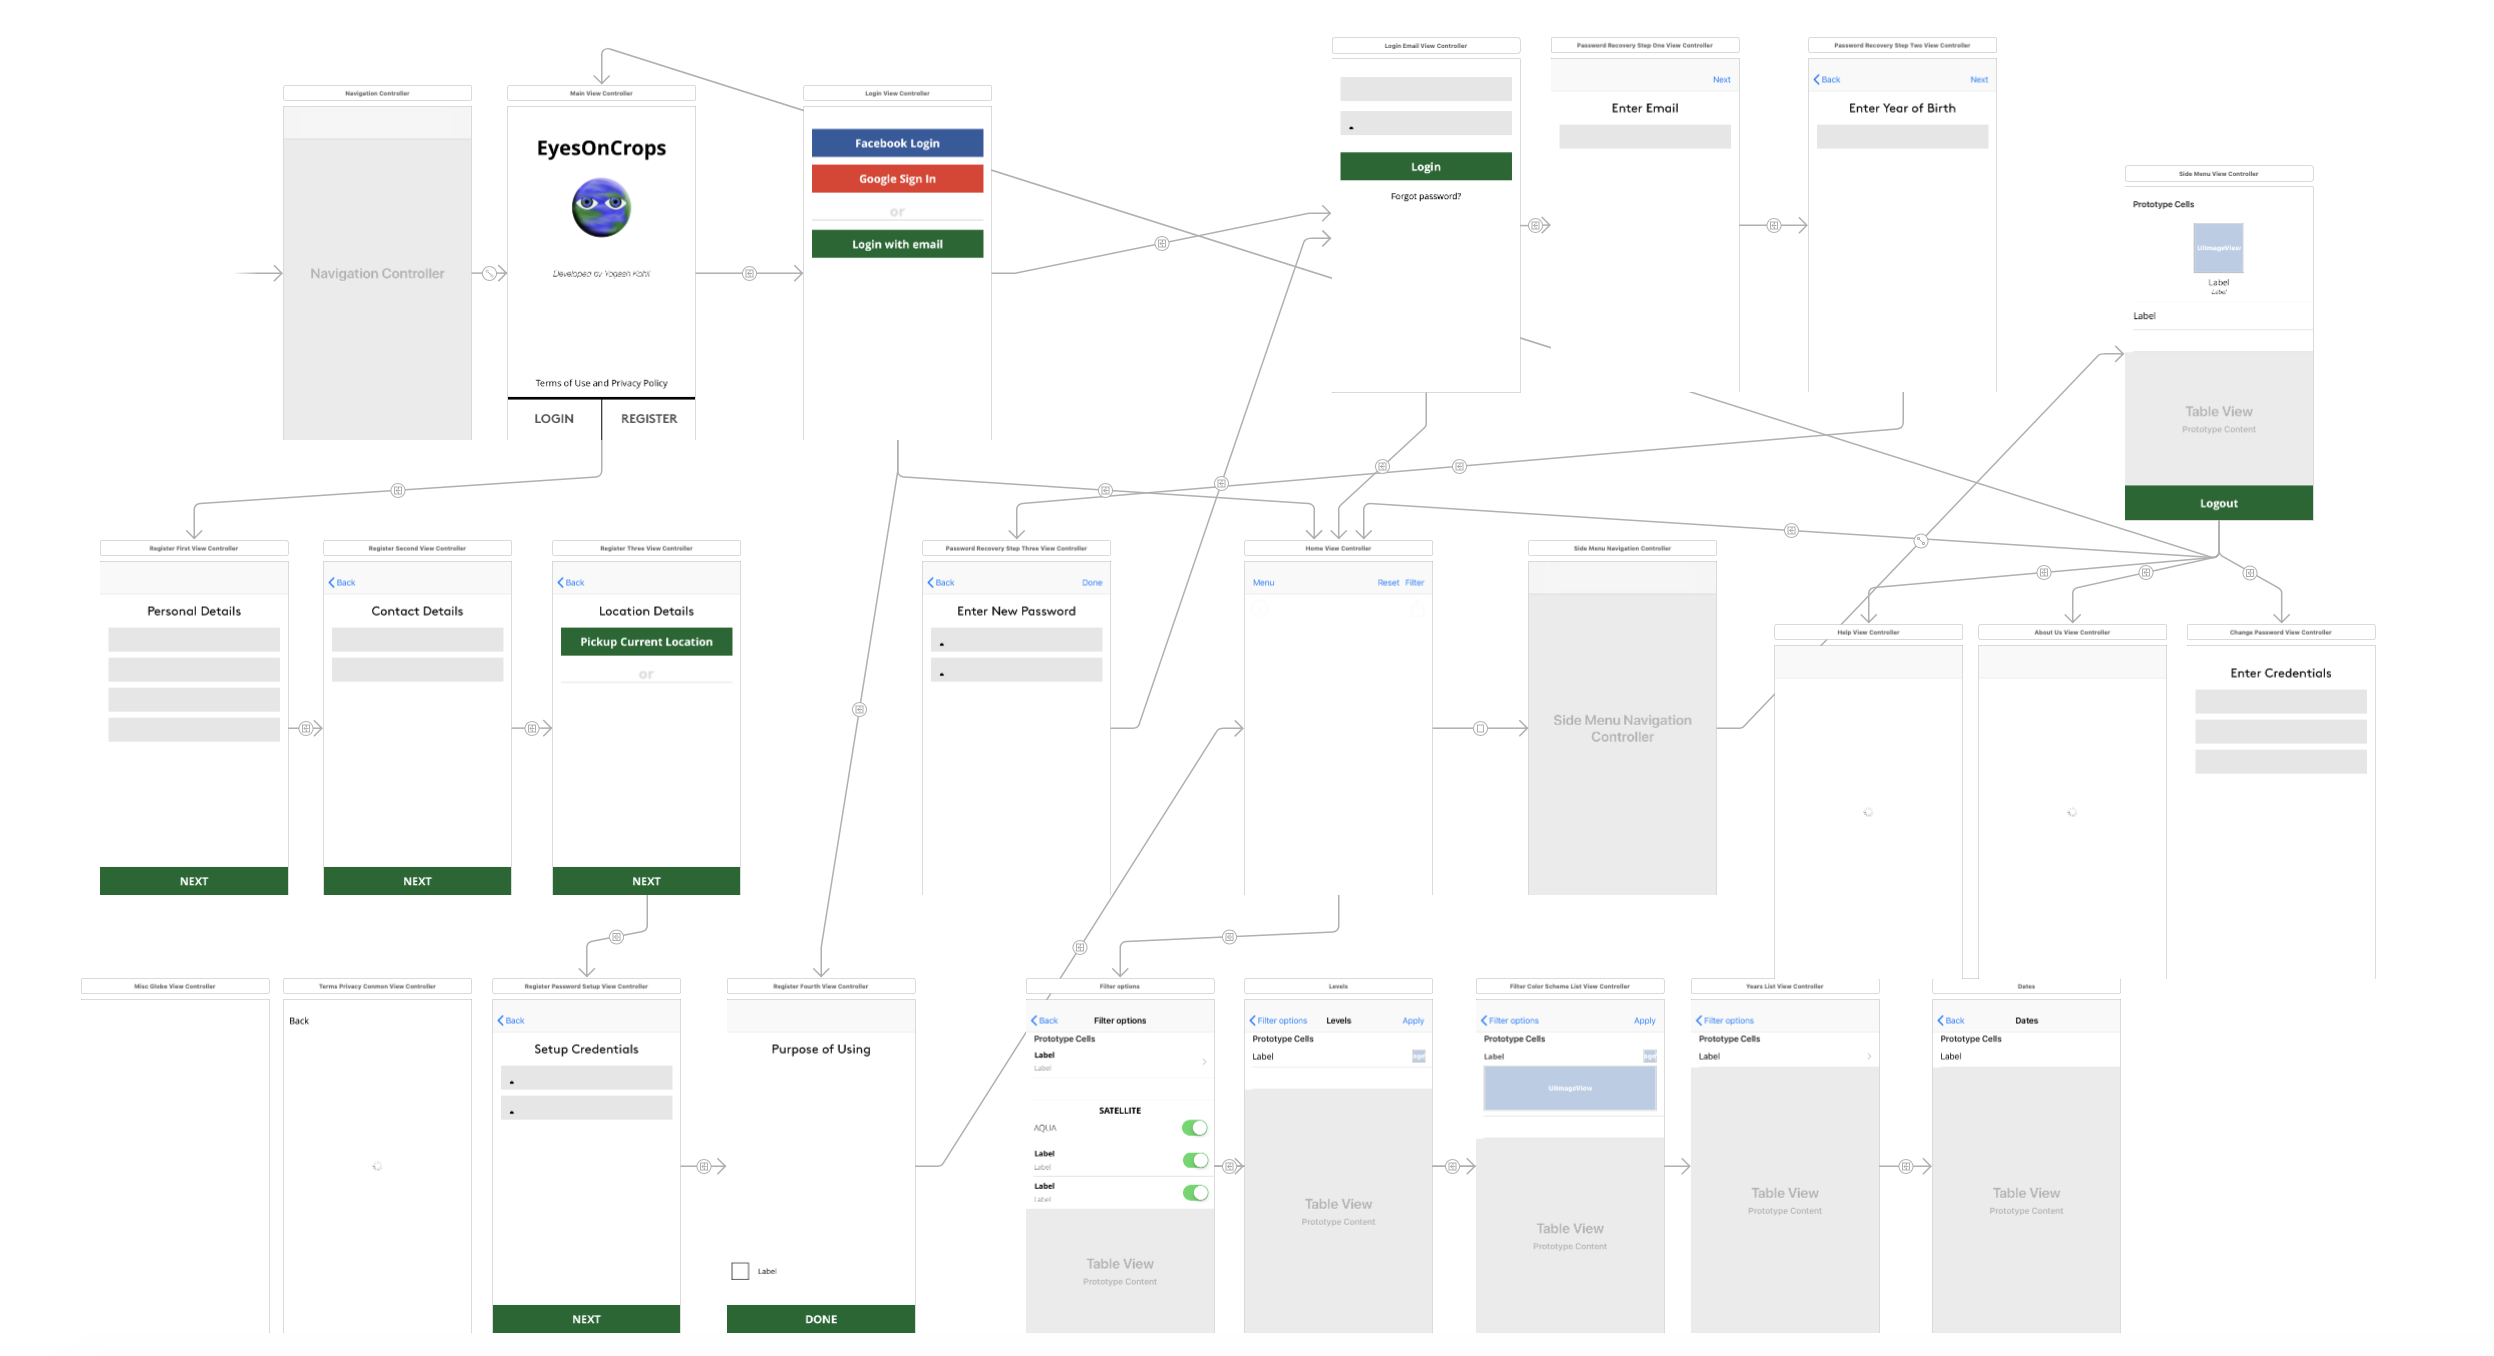
\includegraphics[width=0.95\linewidth]{final/figures/storyboard_final.png}
            \caption{Storyboard of the app}
    \end{figure}
\end{frame}

\begin{frame}
\frametitle{Front-end: Screens and their significance}
EyesOnCrops mainly consists of following:

\begin{itemize}
    \item Register process
    \item Login process
    \item Slide out manu
    \item Home screen
    \item Filter process
\end{itemize}

\end{frame}

\begin{frame}
\frametitle{Front-end: Register process}

    Register via email process is divided into 5 steps:
    
    \begin{itemize}
        \item Personal details
        \item Contact details
        \item Location details
        \item Credentials setup
        \item Purpose of using the app screen
    \end{itemize}
\end{frame}

\begin{frame}
\frametitle{Front-end: Register process screens}
\begin{figure}[H]
            \centering
            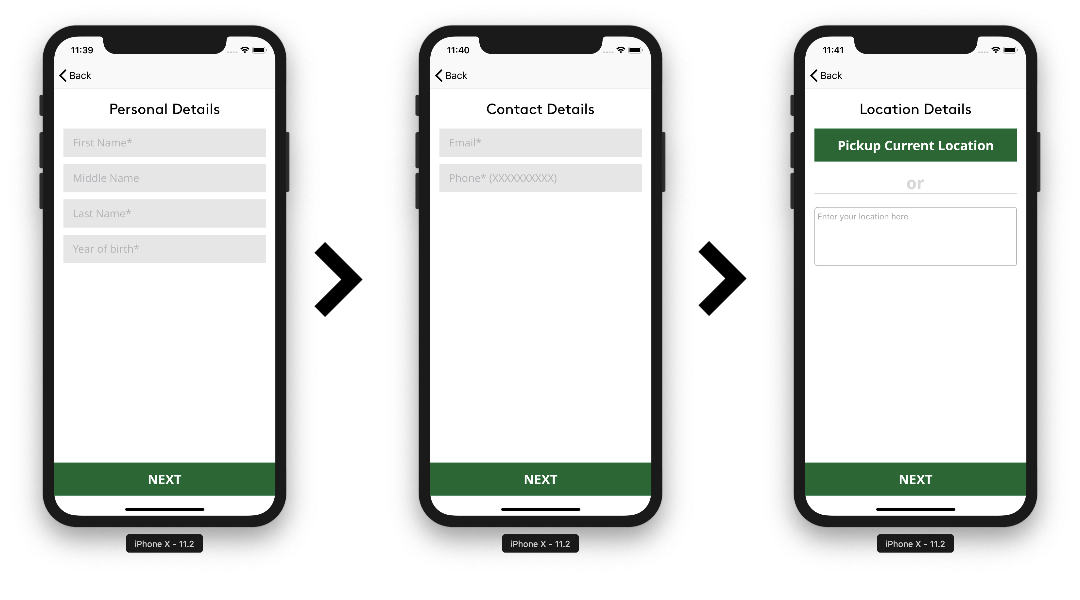
\includegraphics[width=0.95\linewidth]{final/figures/register_1.png}
            \caption{Register screens}
    \end{figure}
\end{frame}

\begin{frame}
\frametitle{Front-end: Register process screens contd.}
    \begin{figure}[H]
            \centering
            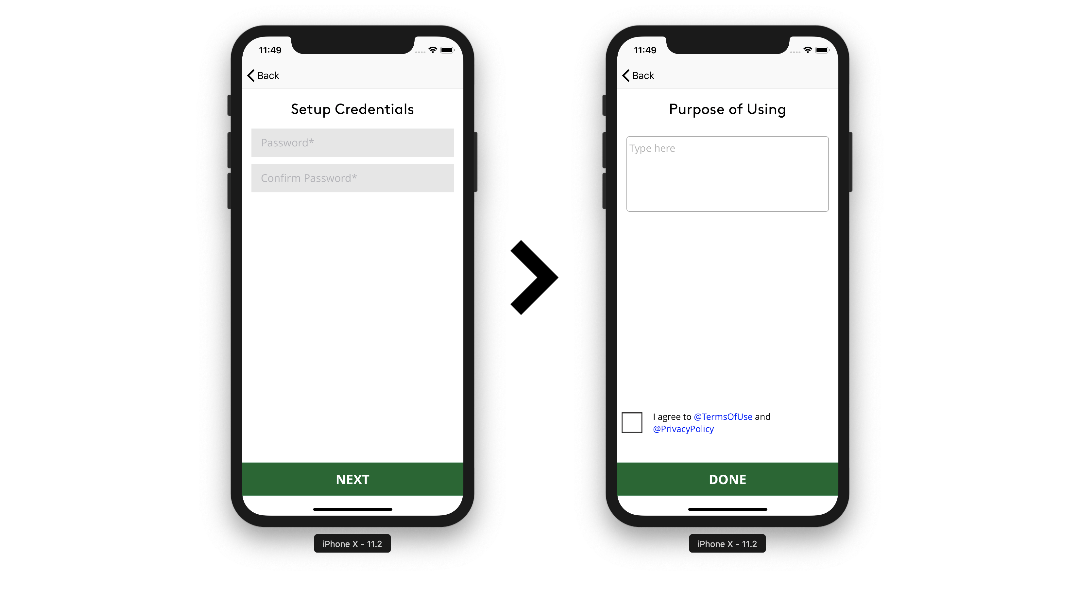
\includegraphics[width=0.95\linewidth]{final/figures/register_2.png}
            \caption{Register screens}
    \end{figure}
\end{frame}

\begin{frame}
\frametitle{Front-end: Login process}

    Login can be achieved via following:
    
    \begin{itemize}
        \item Social login - Facebook \& Gmail
        \item Login via email (if user has registered via email)
    \end{itemize}
\end{frame}

\begin{frame}
\frametitle{Front-end: Login process screens}
    \begin{figure}[H]
            \centering
            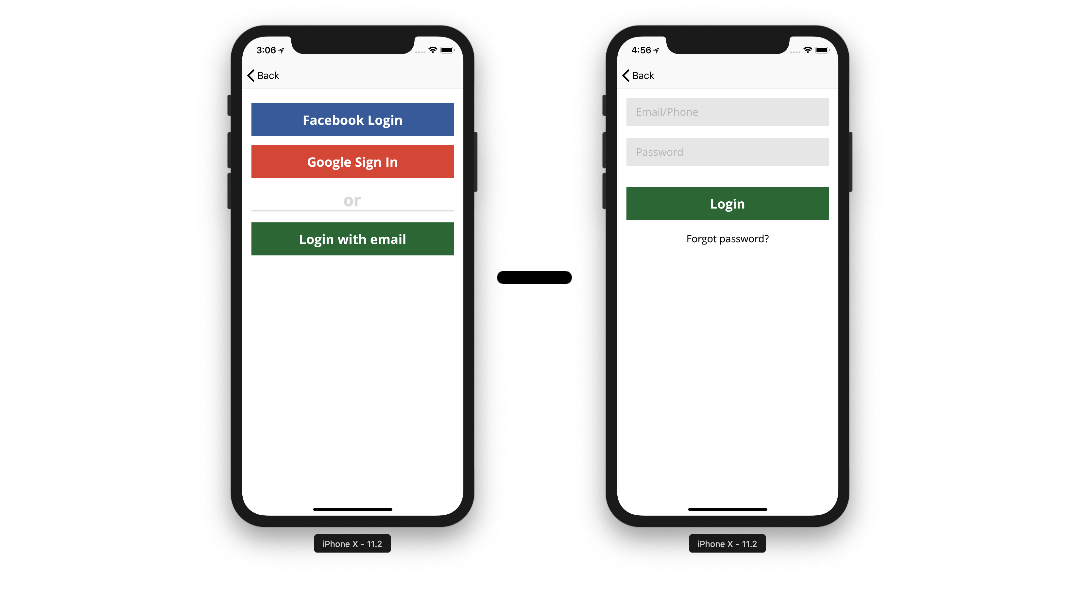
\includegraphics[width=0.95\linewidth]{final/figures/login.png}
            \caption{Login screens - Social and via email}
    \end{figure}
 
\end{frame}

\begin{frame}
\frametitle{Front-end: Slide out menu}
\begin{columns}
\column{0.5\textwidth}

\begin{itemize}
    \item Slide out menu created in the app to make it easy for the user to navigate through the app
    \item Shows the date since user has been registered with us
    \item About us, help sections and logout functionality provided here
\end{itemize}

\column{0.5\textwidth}
\begin{figure}
    \centering
    \begin{minipage}{.5\columnwidth}
    %\includegraphics[width=\linewidth]{ts-compare.png}
    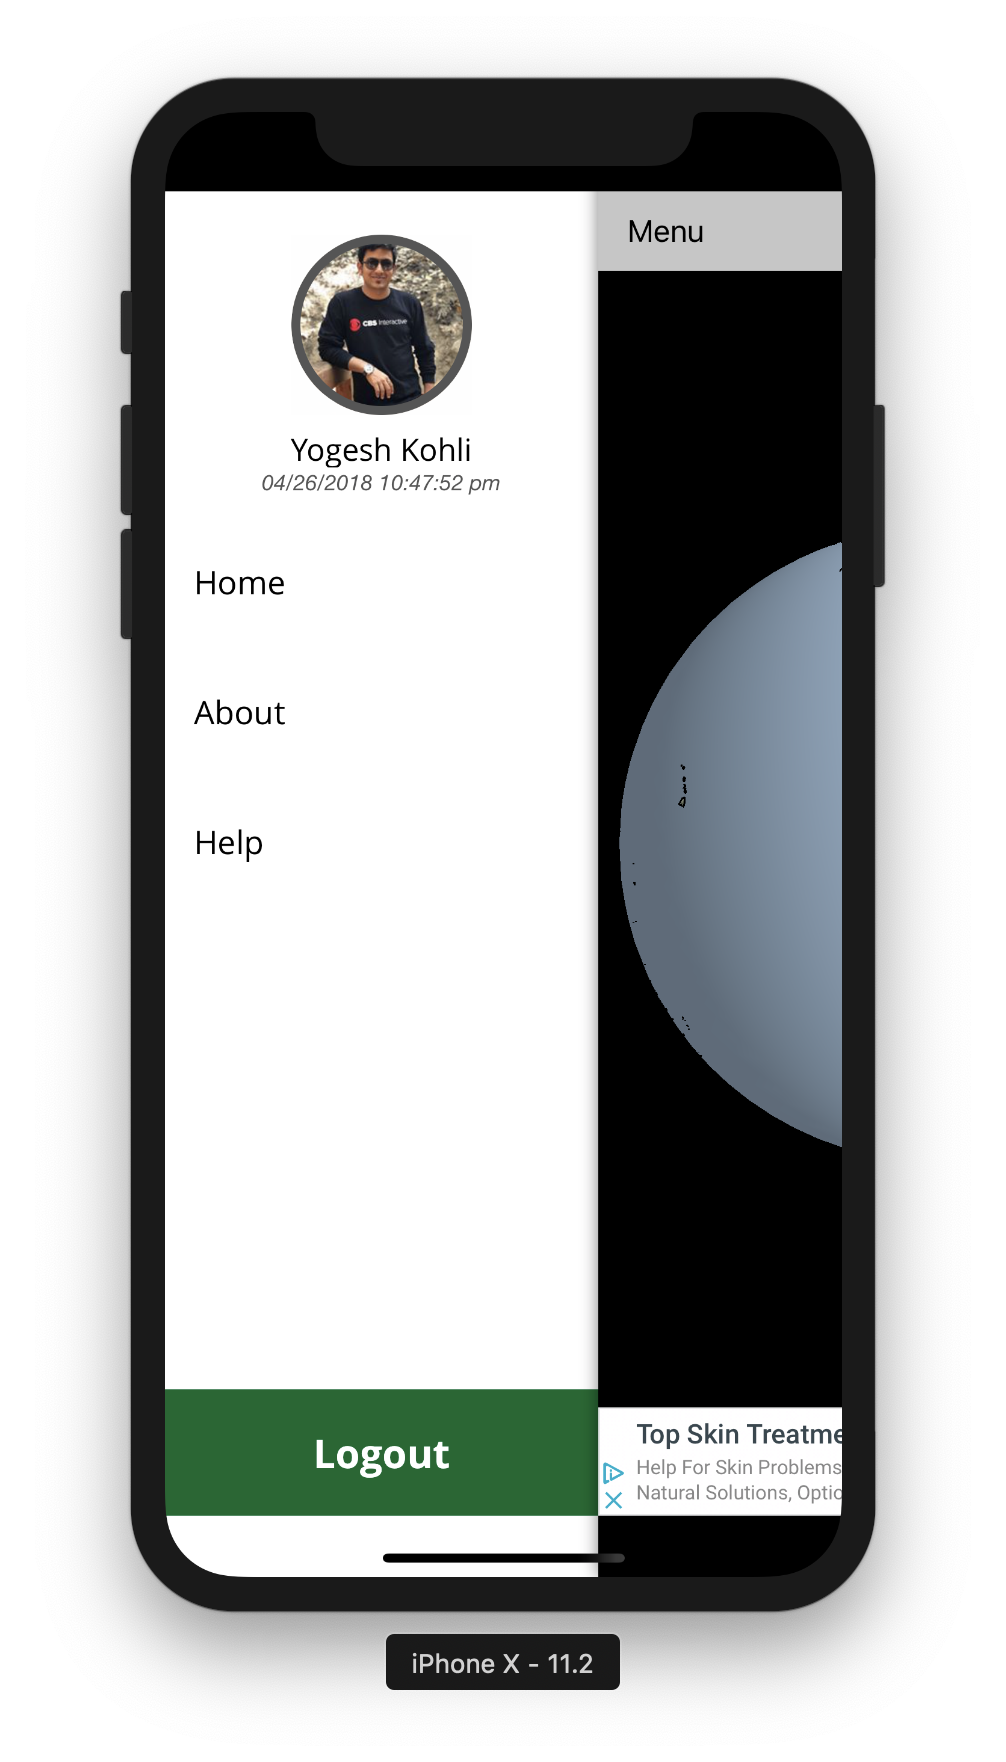
\includegraphics[width=\linewidth]{final/figures/side_menu.png}
    \caption{Slide out menu in the app}
    \end{minipage}
\end{figure}
\end{columns}
\end{frame}

\begin{frame}
\frametitle{Front-end: Home Screen}
   \begin{itemize}
       \item Landing screen once user logs in
       \item It has two modes : Globe view and 2D Map view
       \item Includes Google Ads in the bottom
       \item Most of the time user would be interacting with this screen
   \end{itemize}
\end{frame}

\begin{frame}
\frametitle{Front-end: Home Screen contd.}
   \begin{figure}[H]
            \centering
            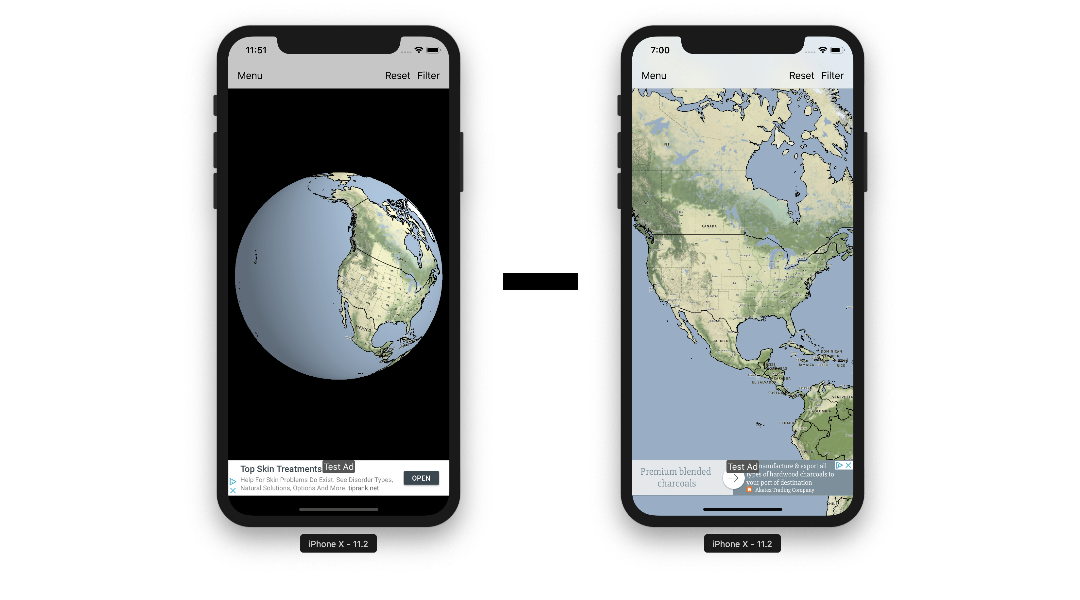
\includegraphics[width=0.95\linewidth]{final/figures/home_modes.png}
            \caption{Home screen with two modes: Globe and Map view}
    \end{figure}
\end{frame}


\begin{frame}
\frametitle{Front-end: Filter process}
\begin{columns}
\column{0.5\textwidth}

 \begin{itemize}
       \item Data type: NDVI / Anomaly
       \item Year and date selection filter
       \item Admin level 0, 1 and 2 filter
       \item Color scheme filter
   \end{itemize}

\column{0.55\textwidth}
\begin{figure}
    \centering
    \begin{minipage}{.5\columnwidth}
    %\includegraphics[width=\linewidth]{ts-compare.png}
    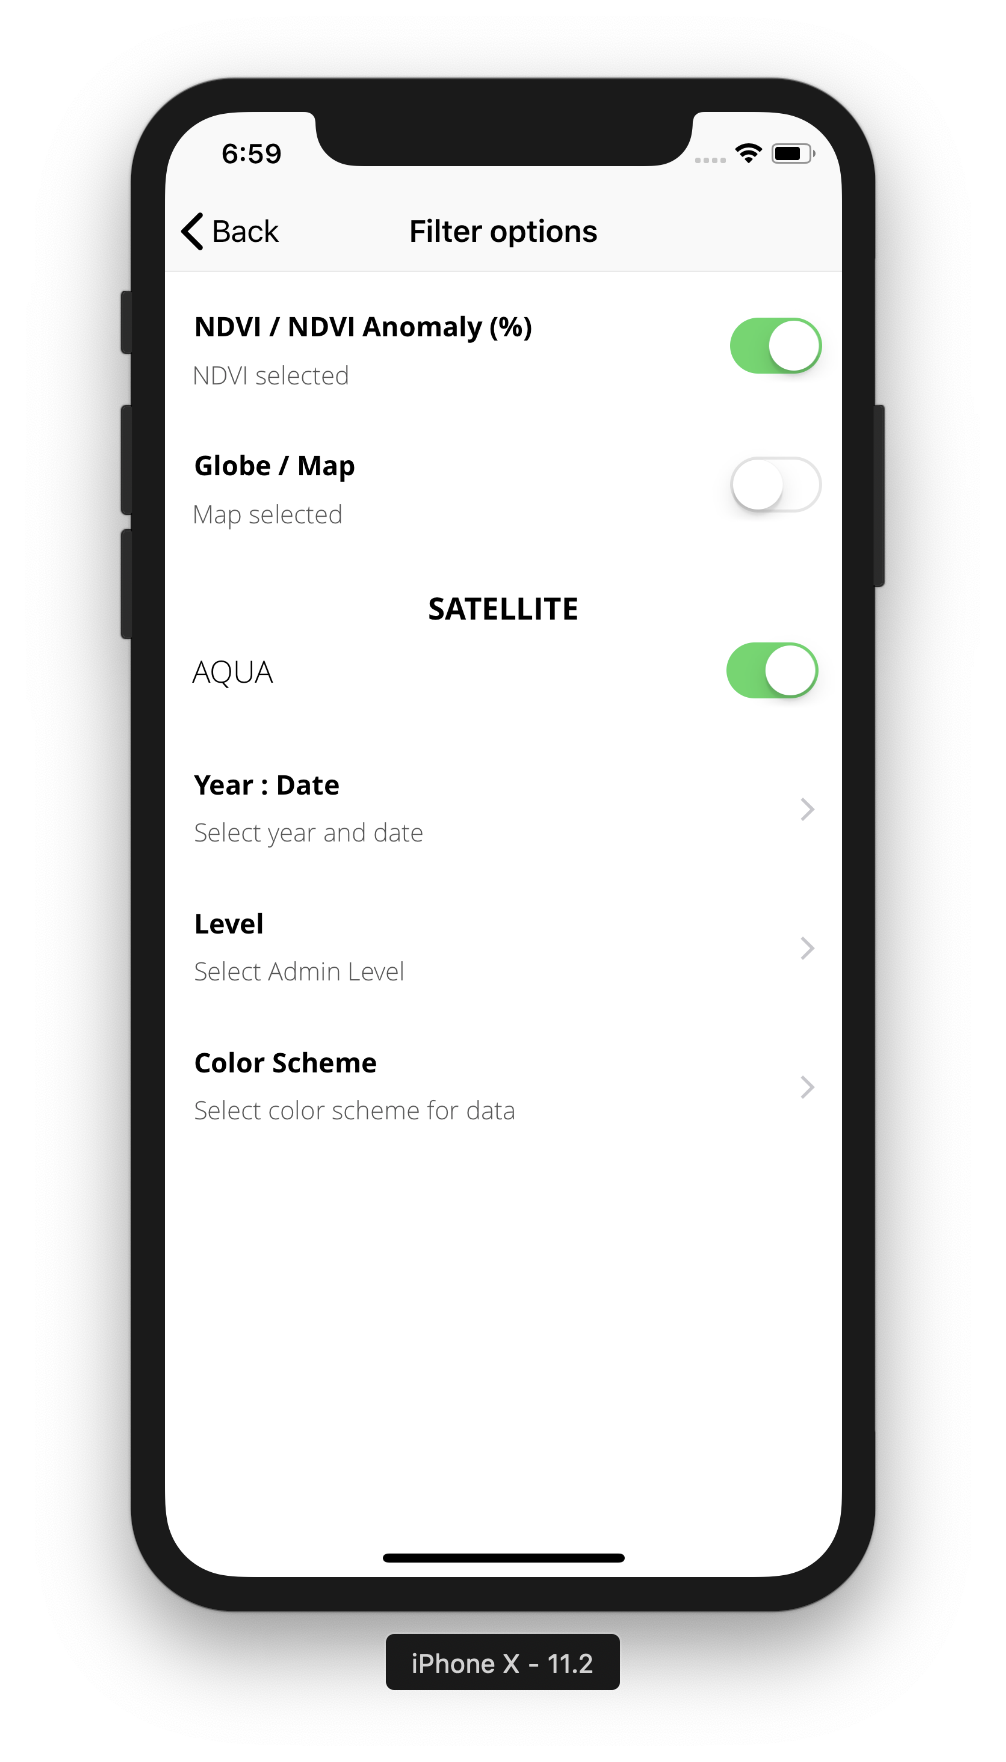
\includegraphics[width=\linewidth]{final/figures/filter.png}
    \caption{Filter screen}
    \end{minipage}
\end{figure}
\end{columns}
\end{frame}


\begin{frame}
\frametitle{Front-end: Filter process: Year and date selection screen}
    \begin{figure}[H]
            \centering
            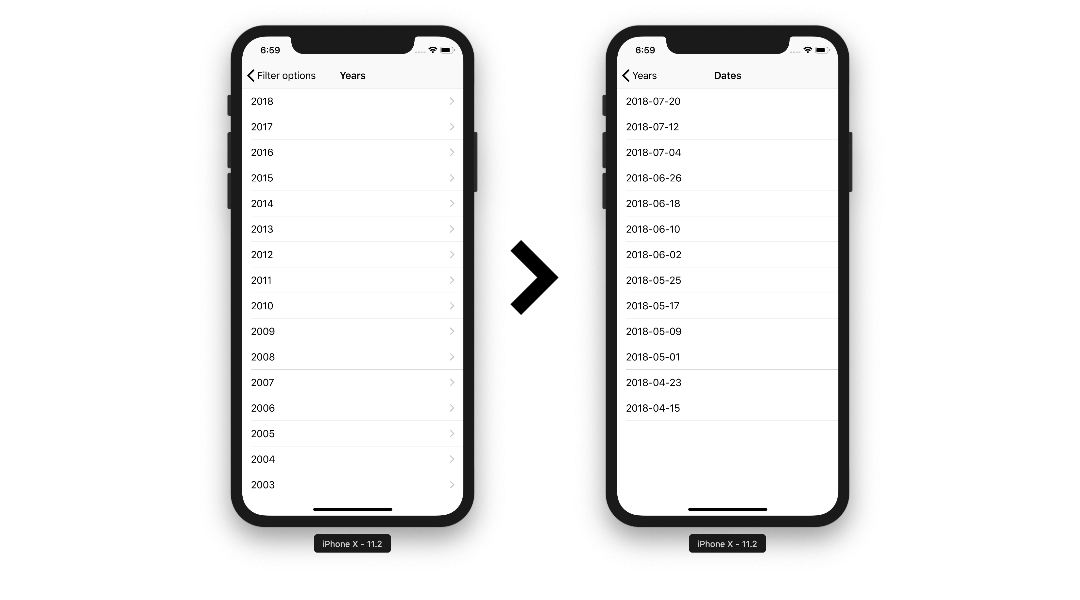
\includegraphics[width=0.95\linewidth]{final/figures/filter_year.png}
            \caption{Filter: Year and date selection}
    \end{figure}
\end{frame}

\begin{frame}
\frametitle{Front-end: Filter process:  Admin levels}

    Admin levels describe how the data will be displayed on the home screen.

   \begin{itemize}
       \item level 0: country wise data - One mean value per country
       \item level 1: state wise - one value per state
       \item level 2: eco-district wise - one value per district
   \end{itemize}
\end{frame}

\begin{frame}
\frametitle{Front-end: Filter process: Color scheme selection}
\begin{columns}
\column{0.5\textwidth}

 \begin{itemize}
       \item Different color schemes available
       \item Another way of visualizing the data in a different color palette. 
   \end{itemize}

\column{0.55\textwidth}
\begin{figure}
    \centering
    \begin{minipage}{.5\columnwidth}
    %\includegraphics[width=\linewidth]{ts-compare.png}
    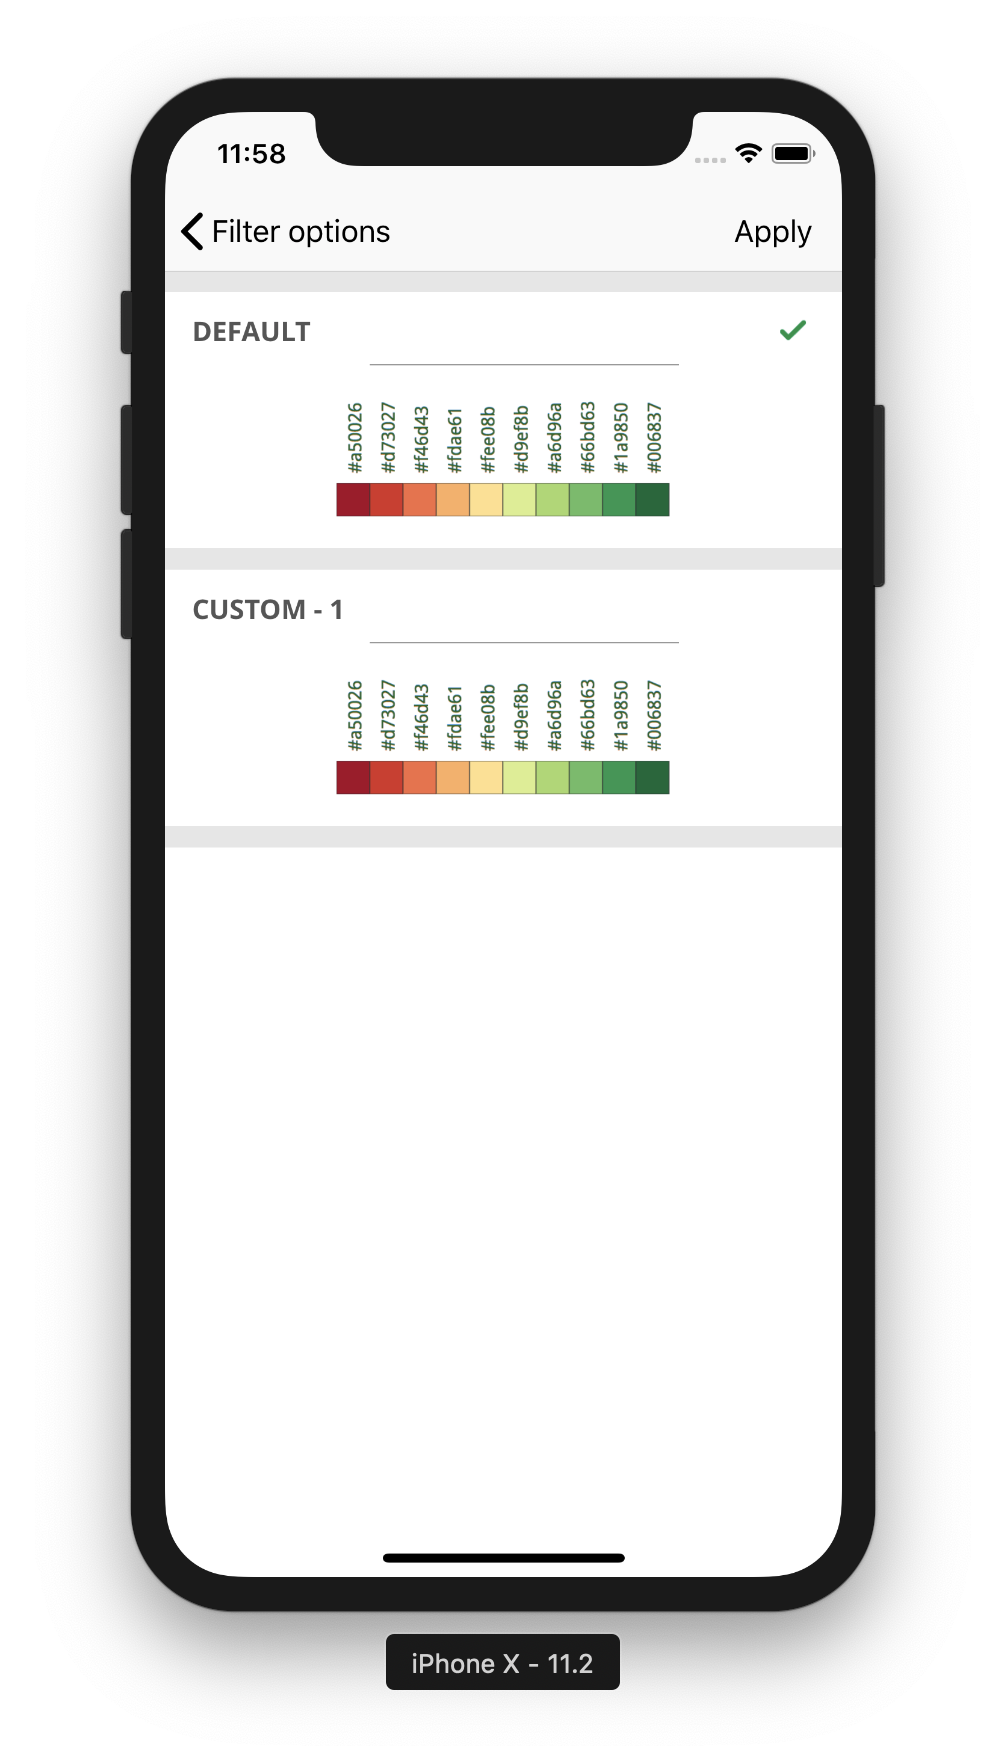
\includegraphics[width=\linewidth]{final/figures/color_scheme.png}
    \caption{Filter: Color scheme selection screen}
    \end{minipage}
\end{figure}
\end{columns}
\end{frame}


\begin{frame}
\frametitle{Back-end process}

   \begin{itemize}
       \item Getting the data from NASA's server and storing it in database
       \item Web services required for JSON parsing between database and the frontend coded in PHP
   \end{itemize}
\end{frame}


\begin{frame}
\frametitle{Back-end: Getting data from NASA's server}
\begin{itemize}
    \item Python script to accomplish this
    \item Reads the data from NASA's server without decompressing the zip file
    \item Only district level data has been stored to prevent redundancy because state and country data includes district level data
\end{itemize}
\end{frame}



\begin{frame}
\frametitle{Back-end: PHP web services for JSON parsing}
\begin{itemize}
    \item Python script to accomplish this
    \item Reads the data from NASA's server without decompressing the zip file
    \item Only district level data has been stored to prevent redundancy because state and country data includes district level data
\end{itemize}

\begin{itemize}
    \item dbcon.php: database connection
    \item credentials.php: register \& login services
    \item get\_data.php: year, date and ndvi/anomaly data services
    \item analysis.php: mean, standard deviation and for svd formatted data calculations
\end{itemize}

\begin{figure}
    \centering
    \begin{minipage}{.5\columnwidth}
    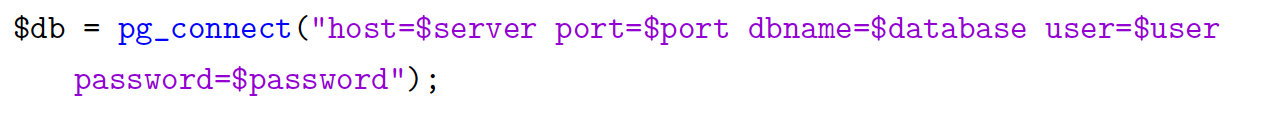
\includegraphics[width=1.0\linewidth]{final/figures/php_dbcon.png}
    \caption{database connection function for PostgreSQL written in PHP}
    \end{minipage}
\end{figure}
\end{frame}


\begin{frame}
\frametitle{Using the application}
\begin{itemize}
    \item Select any filter
    \item Tap on year list and then select date of specific year
    \item Tap on any country/region on the map or globe view to visualize the data.
\end{itemize}
\end{frame}

\begin{frame}
\frametitle{Using the app: Admin level 0: Country wise}
\begin{columns}
\column{0.5\textwidth}

 \begin{itemize}
       \item mean value calculated for the country on specific date
       \item mask mapping of country according to the mean value.
   \end{itemize}

\column{0.55\textwidth}
\begin{figure}
    \centering
    \begin{minipage}{.5\columnwidth}
    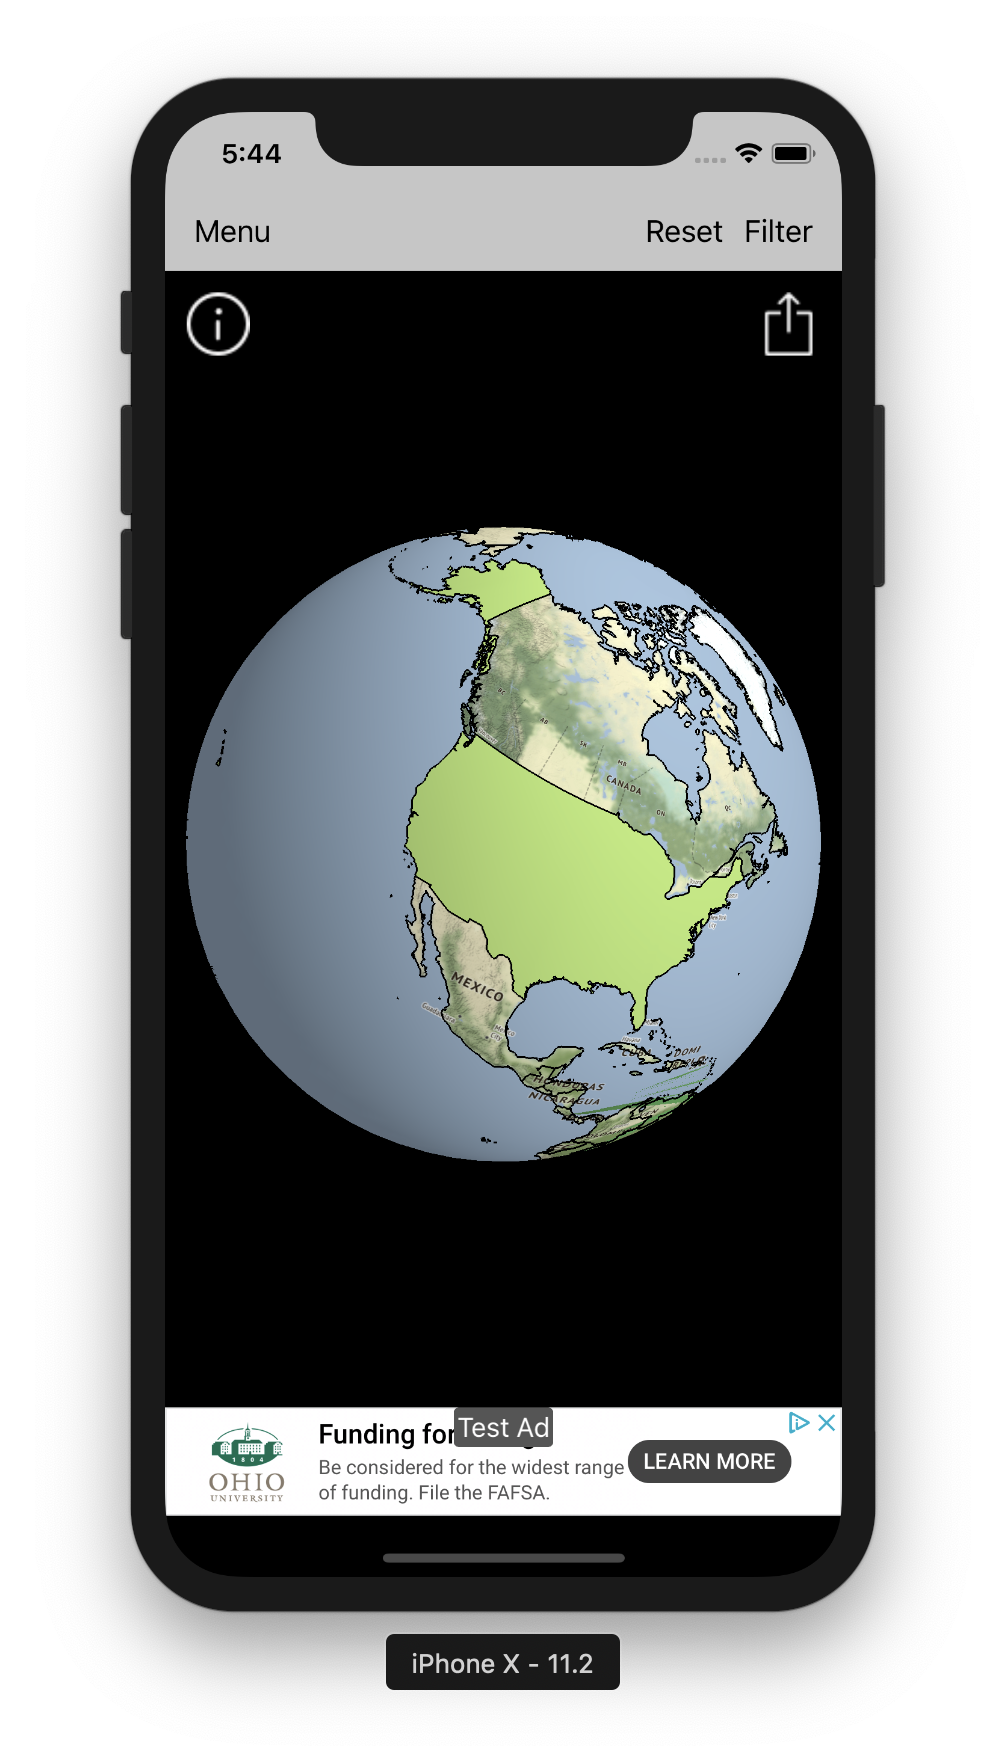
\includegraphics[width=1.0\linewidth]{final/figures/admin_level_0_a.png}
    \caption{United States for 11/11/2017}
    \end{minipage}
\end{figure}
\end{columns}
\end{frame}

\begin{frame}
\frametitle{Using the app: Admin level 1: State wise}
\begin{columns}
\column{0.5\textwidth}

 \begin{itemize}
       \item mean value calculated for every state of the country on specific date
       \item mask mapping of states according to the mean value.
   \end{itemize}

\column{0.55\textwidth}
\begin{figure}
    \centering
    \begin{minipage}{.5\columnwidth}
    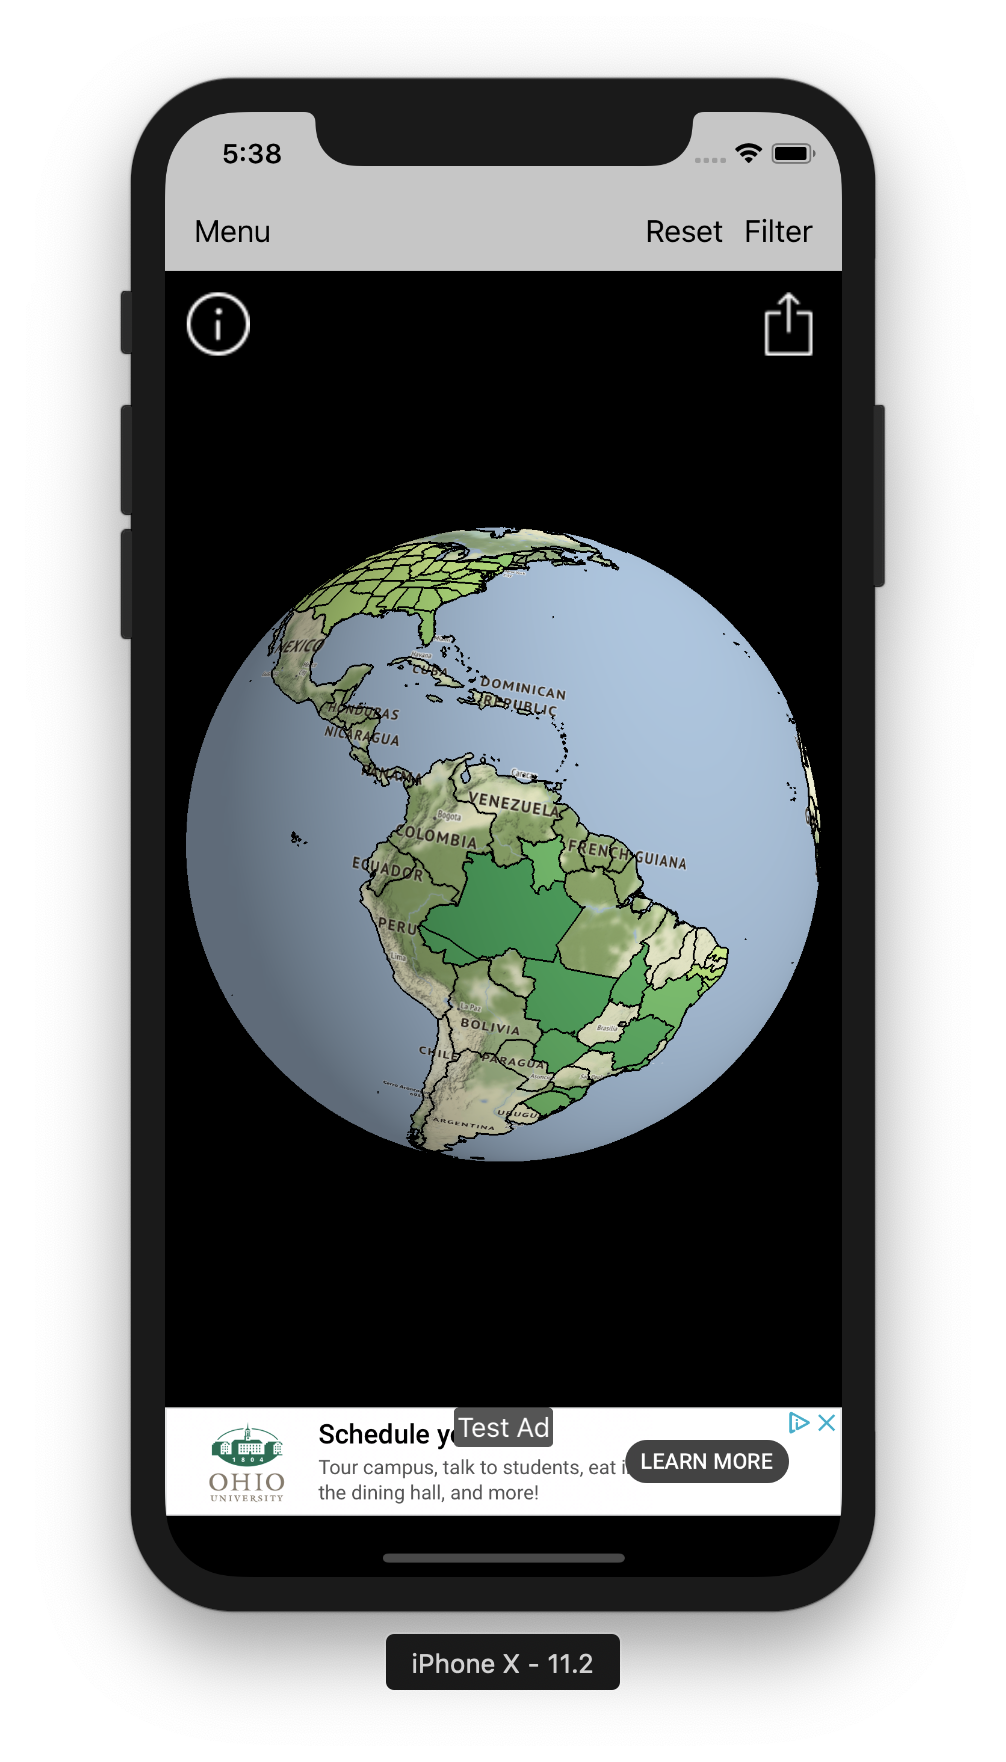
\includegraphics[width=1.0\linewidth]{final/figures/admin_level_1_b.png}
    \caption{United States and Brazil for 11/11/2017}
    \end{minipage}
\end{figure}
\end{columns}
\end{frame}

\begin{frame}
\frametitle{Using the app: Admin level 2: Eco-district wise}
\begin{columns}
\column{0.5\textwidth}

 \begin{itemize}
       \item mean value calculated for every district of the country on specific date
       \item mask mapping of districts according to the mean value.
   \end{itemize}

\column{0.55\textwidth}
\begin{figure}
    \centering
    \begin{minipage}{.5\columnwidth}
    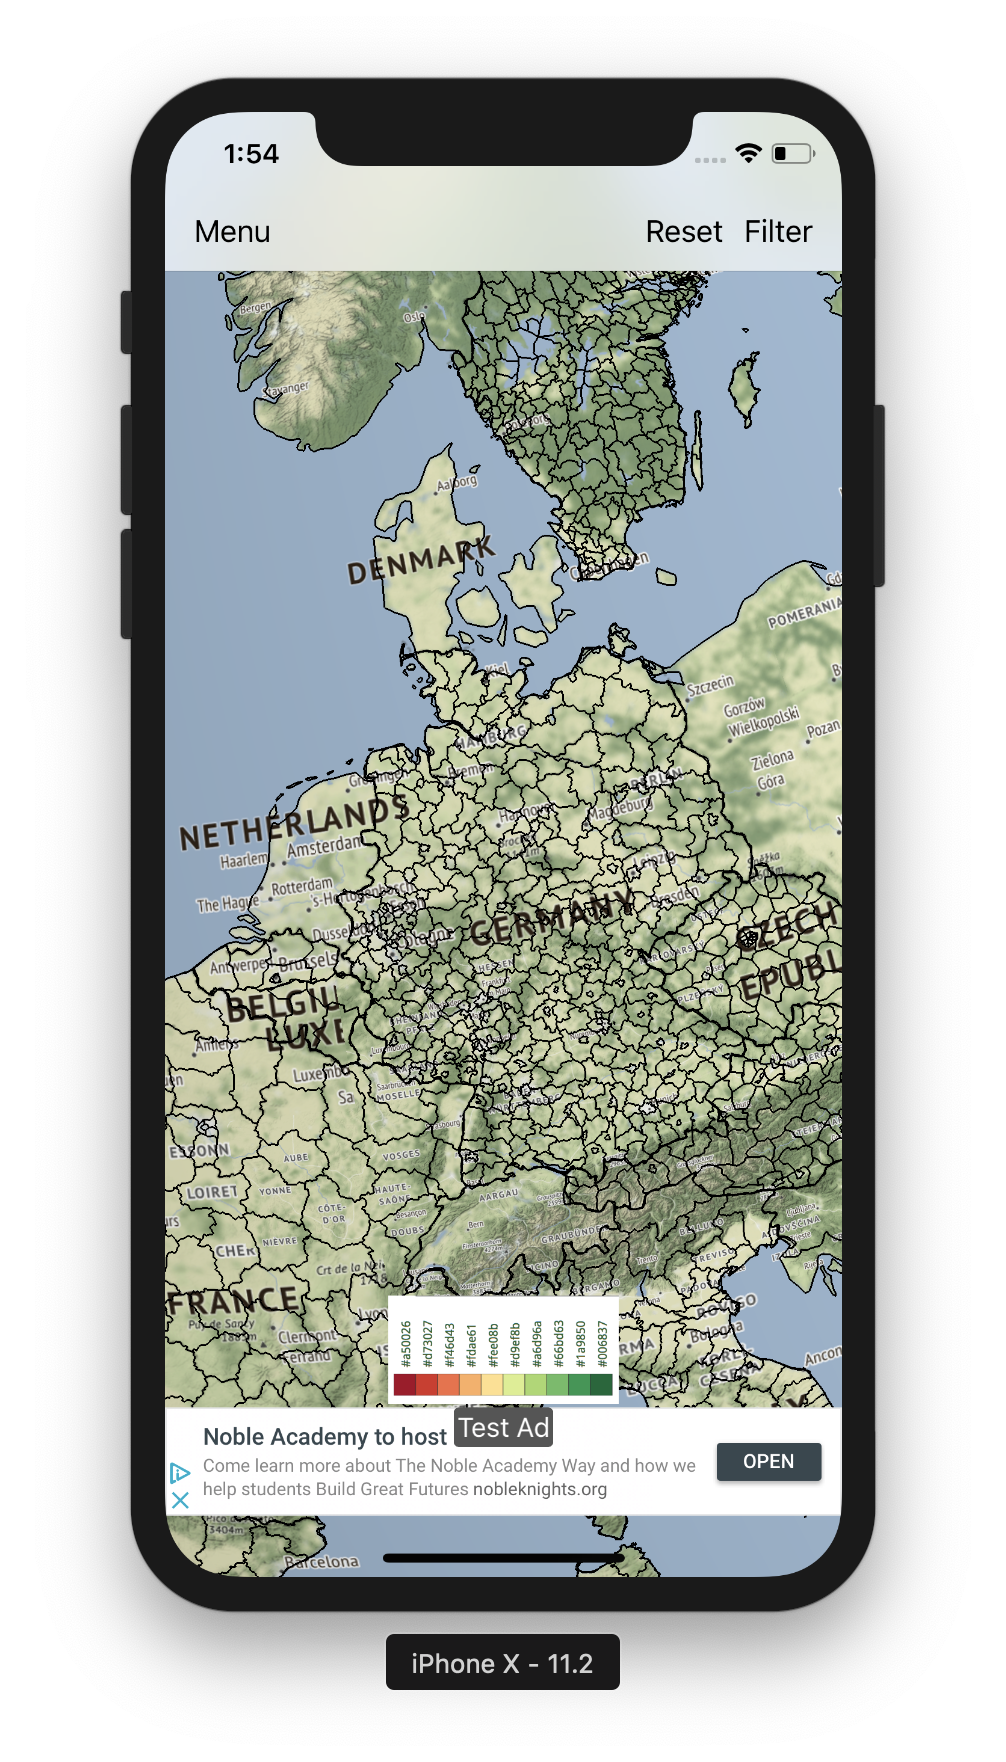
\includegraphics[width=1.0\linewidth]{final/figures/admin_level_2.png}
    \caption{Admin level 2: eco-district level}
    \end{minipage}
\end{figure}
\end{columns}
\end{frame}


\begin{frame}
\frametitle{Analysis}
\begin{itemize}
    \item Data downloading/exporting via email
    \item Mean \& Standard deviation
    \item SVD Analysis
\end{itemize}
\end{frame}


\begin{frame}
\frametitle{Analysis: Data downloading}

\end{frame}